In this section we will provide and overview of the relevant background and context for this thesis. First introducing the software engineering lifecycle and the rising role of GenAi/LLMs in it. The Second part showcases the evolution and state of APR and explores existing approaches.

\section{Software Engineering}
In the follwing section introduces the software engineering lifecycle, the role of code hosting platforms, and the importance of Continuous Integration and Continuous Deployment (CI/CD) in modern software development.
\subsection{Software Development Lifecycle}
Engineering Software is complex and including multiple stages. For structuring this work diffrent Software Developemnt Lifecycle Models have been introduced. Software Development Lifecycle Models evolve constantly to adapt to the chanign needs of creating software. The most promising and widely used model is the Agile Software Development Lifecycle \cite{rupareliaSoftwareDevelopmentLifecycle2010}.

The Agile lifecycle brings an interative approach to development, focusing on collaboration, feedback and adaptivity. The Goal frequent delivery of small functional features of software, allowing for continuous improvement and adaptation to changing requirements. Agile can be used with multiple frameworks like Scrum or Kanban but follows a similar approach. \cite{rupareliaSoftwareDevelopmentLifecycle2010}.

\begin{figure}[htbp]
    \centering
    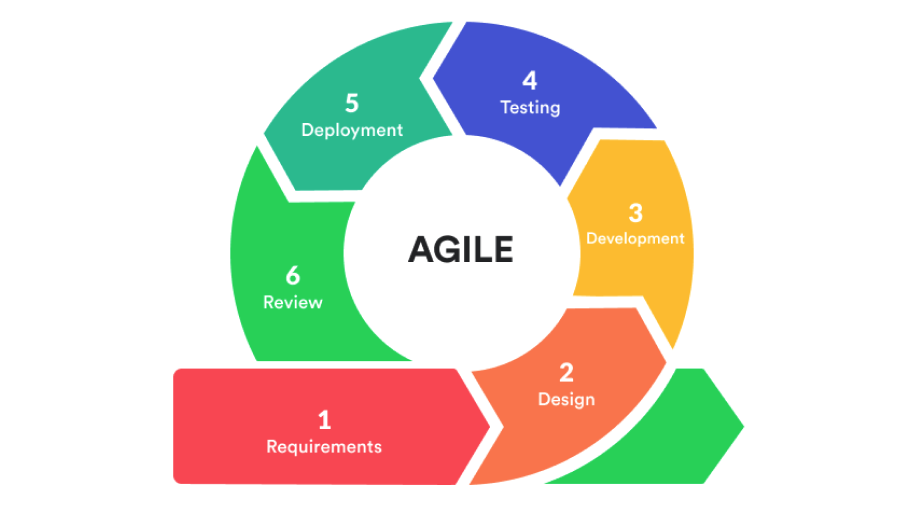
\includegraphics[width=0.8\textwidth]{images/agile-cycle.png}
    \caption{Agile Software Development Lifecycle}
    \label{fig:agile-cycle}
\end{figure}

A Agile Software Development Lifecycle iteration consists of several key stages like in Figure starting with planning phase where requirements for the iterartion are gathered and pritorized.

Since agile focuses adaptivity arising bugs can alter iterations if priotirised and therefore slow down delivery of features. APR is supposed to help with this problem by accelerating the process of fixing bugs.
---explain how bugs are handled

Software development is moving towards lightly coupled microsversives which results in more repositories which are smaller in scale tailored towards a specialzed domain. This trend is driven by the need for flexibility, scalability, and faster development cycles. Smaller code repositories allow teams to work on specific components or services independently, reducing dependencies and enabling quicker iterations. This approach aligns with modern software development practices, such as microservices architecture and agile methodologies.
With this trend developers work on multiple projects at the same time, which can lead to more interrupptions and context swtiching when problems arise and priorities shift.


\subsection{Continuous Integration}

For accelerating the delviery of software in an iteration continous integration has become a standard in agile software development.

\begin{figure}[htbp]
    \centering
    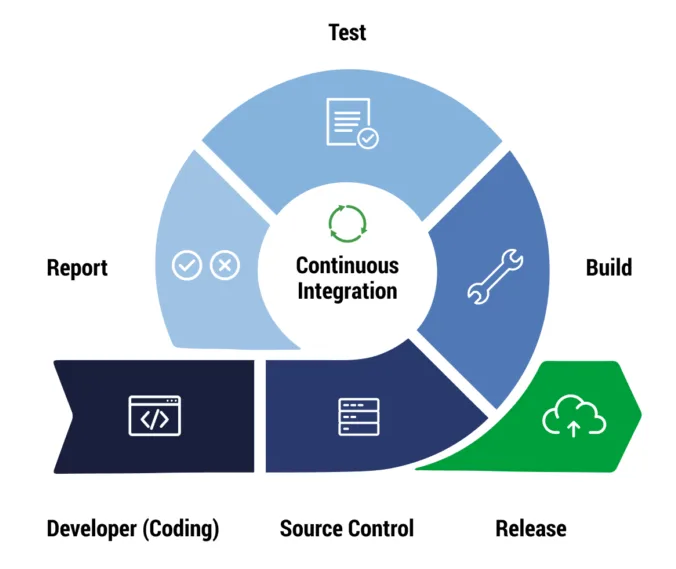
\includegraphics[width=0.8\textwidth]{images/ci-cycle.png}
    \caption{Continuous Integration Cycle}
    \label{fig:ci-cycle}
\end{figure}

Continuous Integration (CI) allows for frequenct code integration into a code repository. Ci can integrate steps like automated building and testing into the development resulting in rapid feedback right where the changes commited to the shared reposirotry.

Althought CI bring a lot of potential to development it can also have problemswhich can be long build durations and high maintance

CI supports aspects like fast delivery, fast feedback, enhanced collaboration which are ciritcal for agile software development. \cite{ugwuezeContinuousIntegrationDeployment2024}

\subsection{Software Project Hosting Platforms}
Software projects are hosted on platforms like Github or gitlab. With Github being the most popular and most used \cite{} These platforms provides tools and feature for the complete software development lifecycle. Project hosting, verssion control, bug and issue tracking, project management, backups, collaboration, and documentation. \cite{abrahamssonAgileSoftwareDevelopment2017}

GitHub has features like Issue tracking for requiremtns and planning with issues looking like this: \cite{githubdoc}
---image of issue
has title, description, comments, labels and mroe assioicated information

also provides a manged soltution for integrating CI into reposiries by writing workflows in YAML files called Github Actions. The pipeliens can run on github hosted runners or self hosted runner. A workflow can be triggered by one or more event. One or more jobscan be executed on a provided runner maschiene. A job can consist of multiple steps. \cite{Workflows}
\begin{figure}[htbp]
    \centering
    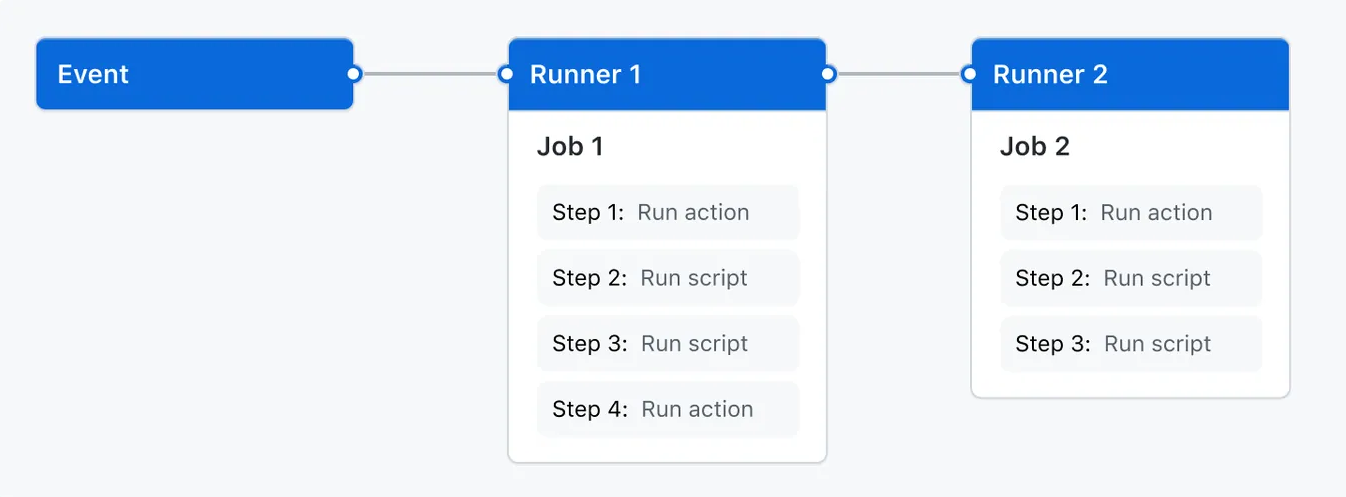
\includegraphics[width=0.8\textwidth]{images/overview-actions-simple.png}
    \caption{Simple Action}
    \label{fig:simple action}
\end{figure}

Since constant feedback and reviews of code play an imporatnt role in agile workflows github also provides a pull request feature. Pull Requests allow for proposal of changes to the codebase, with an integrated review process which allows for collaboration and review before changes are integrated into the production codebase.
Code changes are displayed in a diff format allowing reviews to see and dig into the changes made.
This process is essential for maintaining code quality and ensuring that changes are validated before being merged. \cite{githubdoc}

\section{Generative Ai in Software Development}

\subsection{Generative AI and Large Language Models}
Gen ai is subfield of Ai

LLms work using human langague data

relatively new advancement are AI Agents which let LLMs interact with the environment and plan their actions

\subsection{Generative AI in Software Development}
%TODO Table of models? also mention open source?
Generative AI is reshaping software development by autoamting various tasks. Modern large language models have billions of paramters, are pre-tained on massive codesbases which results in extraordinary capbilites in this area  \cite{chenUnveilingPitfallsUnderstanding2025}.
Tools like Github Copilot, OpenAI Codex, and ChatGPT have become popular in the software development community, providing developers with AI-powered code suggestions and completions for dirrent tasks \cite{bhargavmallampatiRoleGenerativeAI2025}. These tools get applied in various stages of the software development lifecycle, including requirement engineering, code generation, debugging, refactoring, and testing \cite{houLargeLanguageModels2024, puvvadiCodingAgentsComprehensive2025,
    bhargavmallampatiRoleGenerativeAI2025 }. LLms can generate code in diffrent programmming languages. With python being the to supoorted \cite{}
By using LLMs to enhance these tasks developemtn cycle times can be reduced by up to 30 percent \cite{bhargavmallampatiRoleGenerativeAI2025,kalliamvakouResearchQuantifyingGitHub2022}. Furthermore these tools have postive impacts like improving developer statisfaction and reducing congintive load \cite{kalliamvakouResearchQuantifyingGitHub2022}.

Although Generative Ai get adpoted really quickly in many areas of software development this transition still faces callenges and limitations.
LLMs have issues working on tasks that are outside their scope of training or require specific domain knowledge \cite{houLargeLanguageModels2024}.
Additionally LLMs have limited context windows, which can lead to challenges when working with large codebases or complex projects where context windows are too small ofr true contextual or requiremtns understanding \cite{bhargavmallampatiRoleGenerativeAI2025}.
When generating code LLMs can produce incorrect or insecure code, which can lead to further bugs and vulnerabilities in the software \cite{houLargeLanguageModels2024}.
Generating content or code with LLMs based on training data raises questions about ownership, reposinisbily and intellectual property rights.
When it comes to security geneerating code using prompts is vunerable to prompt injection, where unintended instructions are injected at some point and can lead to production of harmful code \cite{}

\cite{bhargavmallampatiRoleGenerativeAI2025, houLargeLanguageModels2024}.
When generating code based on training data interlecutal property issues arise  \cite{sauvolaFutureSoftwareDevelopment2024}


recently research and companies is looking into developing solutions which integration LLMs into exisitng software development practices and workflows  \cite{puvvadiCodingAgentsComprehensive2025, dohmkeGitHubCopilotMeet2025, ntroducingCodex, sauvolaFutureSoftwareDevelopment2024}.

recently more attention is given to itnergration of AI/ML into CICD
\cite{mohammedAIDrivenContinuousIntegration2024}

\section{Automated Programm Repair}

Automated Program Repair (APR) is software that helps detect and repair bugs in code with minimal human intervention. This field has also benefited of the rapid advancements in AI.

APR system are supposed to take over the process of fixing bugs therefore making more time for developers to focus on more relevant work. \cite{houLargeLanguageModels2024}

Specific bugs can be fixed using a resulting patch from an APR system. For creating working patches APR takes a 3 stage approach: First localizing the bug. Then repairing the bug, in the end validation decides where the bug will be passed on.\cite{}

In this section we will provide an overview of the evolution of APR, related work, and the current state of APR systems.

\subsection{Evolution of Automated Program Repair}
We have seen multiple transformations in the field of Automated Program Repair (APR) over the years. This evolution of APR can be categorized into key stages, each marked by significant advancements in techniques and methodologies.

\textbf{Tradtional Approaches:}\\
Prior APR approaches were based on version control history, using the history to roll back to a previous version of the code part, where no issues were present. This approach, while effective in some cases, often lacked the ability to perserve new features. (more like instant rollback)

Tempalte based systems relied on predefined template for transformations of commonly known bugs. Tempaltes applied predefined transformtions to the code based on fixed rules. This Apporach had limited the flexibility and adaptability in a quickly transforming software landscape. \cite{puvvadiCodingAgentsComprehensive2025}

%TODO
Search based repair,

%TODO
Semantic based repair,

One of the most outstanding system is Getafix develop and deployed at Meta \cite{baderGetafixLearningFix2019}

Nevertheless tradional systems face significant limitations in scalability and adaptability, struggling to generalize to new scenarios or unseen bugs, or to adapt to evolving codebases. They often required extensive computational resources or manual effort. \cite{puvvadiCodingAgentsComprehensive2025}


\textbf{The emerge of llm based APR:}
LLM based APR techniques have demonstrated siognificant improvments over all other state of the art technqiues, benfitintting from theor coding knowledge \cite{hossainDeepDiveLarge2024}For that reason LLMs lay the groundwork of a new APR paradigm \cite{chenUnveilingPitfallsUnderstanding2025}.
Common LLMS used for APR include GPT-4, ChatGPT, Codex, CodeLlama, DeepSeek-Coder, and CodeT5 \cite{houLargeLanguageModels2024, yinThinkRepairSelfDirectedAutomated2024,anandComprehensiveSurveyAIDriven2024}.

Using LLMs diffrent Paradigms have emerged and are being actively researched. These paradigms include:

Retrieval-Augmented Approaches repair bugs with the help of retrieving relevant context during the repair process. This approach allows adding external knowledge to the repair process, enhancing the LLM's ability to understand and fix bugs \cite{houLargeLanguageModels2024, yinThinkRepairSelfDirectedAutomated2024}.

Agent based system improve fixing abilites by probiding llms the ability to interact with the code base and the environment, allowing them to plan their actions. These frameworks recosncturct the cognitve processes using multiple Agents that can generate code with the help of multi-step reasoning, usage of tools for  with Envrioments and Tools \cite{}. Examples for that are SWE-Agent \cite{ \cite{yangSWEagentAgentComputerInterfaces2024}}, FixAgent \cite{leeUnifiedDebuggingApproach2024}, MarsCodeAgent \cite{liuMarsCodeAgentAInative2024}, GitHub Copilot.

complex agent arcitectures produce good results espically paired with containerized environments. \cite{puvvadiCodingAgentsComprehensive2025}

Interactive apporaches make use of LLMs dialogue capabilities to equip patch validation with instant feedback. This feedback is used to refine the generated patches trying to archieve better results. This process takes a more dynmaic and iterative approach. \cite{xiaAutomatedProgramRepair2024}

Agentless systems are recent a push towards more lightweight solution, focusing on simplicity and efficiency. These approaches aim to reduce the complexity of APR systems while maintaining effectiveness in bug fixing \cite{xiaAgentlessDemystifyingLLMbased2024}. Furthermore this approach provides clear rails to the LLMS improving the transparency of the bug fixing approach taken.
These Systems have archieved promising results  with low costs \cite{xiaAgentlessDemystifyingLLMbased2024}


% TODO mention codex and copilot??

Common problems currently faced by state of the art APR system are:
Exsiting system are overly complex with limited transparency and control over the bug fixing process.\cite{xiaAgentlessDemystifyingLLMbased2024,puvvadiCodingAgentsComprehensive202, houLargeLanguageModels2024}
Repairing bugs takes a lot of compoutational resources and is time intensive therefore producing significant costs  \cite{sobaniaAnalysisAutomaticBug2023,puvvadiCodingAgentsComprehensive2025}
Repairing bugs is done on benchmarks or in controlled set up envrionments and not integrated into real world software development workflows \cite{meemExploringExperiencesAutomated2024,puvvadiCodingAgentsComprehensive2025}

\subsection{APR benchmarks}
Popualr are Quixbugs small bugs in python , Defects4J for java programs and the hardest: SWE Bench based on real world github issues in python repositories


\subsection{APR in CI Context}

CI allows seemless integration...
this way there is no harmfull code executed on own machiene, its encapsulated mutliple times container in Ci runner
